
%(BEGIN_QUESTION)
% Copyright 2013, Tony R. Kuphaldt, released under the Creative Commons Attribution License (v 1.0)
% This means you may do almost anything with this work of mine, so long as you give me proper credit

Draw connecting wires between the 4-20 mA loop-powered pressure transmitter, the 24 VDC power supply, and the voltmeter to form a complete pressure-measurement ``loop'' circuit:

$$\includegraphics[width=15.5cm]{i02646x01.eps}$$

Also, identify whether each component in this circuit is an electrical {\it source} or an electrical {\it load}.

\underbar{file i02646}
%(END_QUESTION)





%(BEGIN_ANSWER)

This is just one possible solution:

$$\includegraphics[width=15.5cm]{i02646x02.eps}$$

Note how current (shown in the direction of conventional flow) always exits the positive terminal of a source, and always enters the positive terminal of a load.

%(END_ANSWER)





%(BEGIN_NOTES)


%INDEX% Pictorial circuit review (analog signal wiring to loop indicator)

%(END_NOTES)


